% The diagonal argument (generated by figs_c3ch03.py).
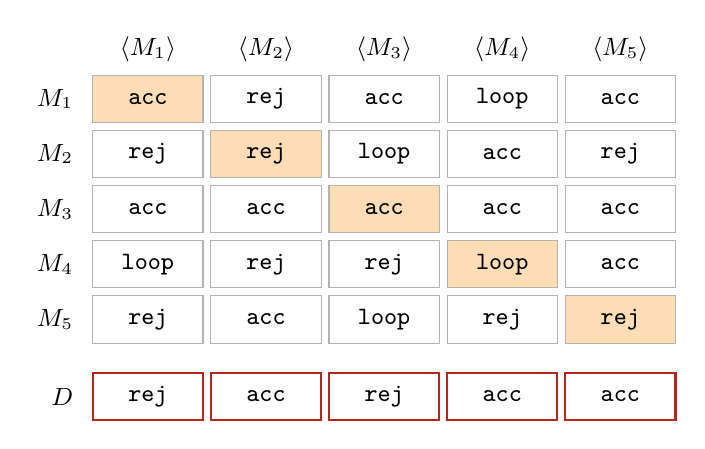
\begin{tikzpicture}[x=15mm,y=7mm,every node/.style={font=\small}]
\node at (1,0.9) {$\langle M_1\rangle$};
\node at (2,0.9) {$\langle M_2\rangle$};
\node at (3,0.9) {$\langle M_3\rangle$};
\node at (4,0.9) {$\langle M_4\rangle$};
\node at (5,0.9) {$\langle M_5\rangle$};
\node[anchor=east] at (0.45,0) {$M_1$};
\node[draw=black!30,fill=BurntOrange!25,minimum width=14mm,minimum height=6mm] at (1,0) {\texttt{acc}};
\node[draw=black!30,fill=white,minimum width=14mm,minimum height=6mm] at (2,0) {\texttt{rej}};
\node[draw=black!30,fill=white,minimum width=14mm,minimum height=6mm] at (3,0) {\texttt{acc}};
\node[draw=black!30,fill=white,minimum width=14mm,minimum height=6mm] at (4,0) {\texttt{loop}};
\node[draw=black!30,fill=white,minimum width=14mm,minimum height=6mm] at (5,0) {\texttt{acc}};
\node[anchor=east] at (0.45,-1) {$M_2$};
\node[draw=black!30,fill=white,minimum width=14mm,minimum height=6mm] at (1,-1) {\texttt{rej}};
\node[draw=black!30,fill=BurntOrange!25,minimum width=14mm,minimum height=6mm] at (2,-1) {\texttt{rej}};
\node[draw=black!30,fill=white,minimum width=14mm,minimum height=6mm] at (3,-1) {\texttt{loop}};
\node[draw=black!30,fill=white,minimum width=14mm,minimum height=6mm] at (4,-1) {\texttt{acc}};
\node[draw=black!30,fill=white,minimum width=14mm,minimum height=6mm] at (5,-1) {\texttt{rej}};
\node[anchor=east] at (0.45,-2) {$M_3$};
\node[draw=black!30,fill=white,minimum width=14mm,minimum height=6mm] at (1,-2) {\texttt{acc}};
\node[draw=black!30,fill=white,minimum width=14mm,minimum height=6mm] at (2,-2) {\texttt{acc}};
\node[draw=black!30,fill=BurntOrange!25,minimum width=14mm,minimum height=6mm] at (3,-2) {\texttt{acc}};
\node[draw=black!30,fill=white,minimum width=14mm,minimum height=6mm] at (4,-2) {\texttt{acc}};
\node[draw=black!30,fill=white,minimum width=14mm,minimum height=6mm] at (5,-2) {\texttt{acc}};
\node[anchor=east] at (0.45,-3) {$M_4$};
\node[draw=black!30,fill=white,minimum width=14mm,minimum height=6mm] at (1,-3) {\texttt{loop}};
\node[draw=black!30,fill=white,minimum width=14mm,minimum height=6mm] at (2,-3) {\texttt{rej}};
\node[draw=black!30,fill=white,minimum width=14mm,minimum height=6mm] at (3,-3) {\texttt{rej}};
\node[draw=black!30,fill=BurntOrange!25,minimum width=14mm,minimum height=6mm] at (4,-3) {\texttt{loop}};
\node[draw=black!30,fill=white,minimum width=14mm,minimum height=6mm] at (5,-3) {\texttt{acc}};
\node[anchor=east] at (0.45,-4) {$M_5$};
\node[draw=black!30,fill=white,minimum width=14mm,minimum height=6mm] at (1,-4) {\texttt{rej}};
\node[draw=black!30,fill=white,minimum width=14mm,minimum height=6mm] at (2,-4) {\texttt{acc}};
\node[draw=black!30,fill=white,minimum width=14mm,minimum height=6mm] at (3,-4) {\texttt{loop}};
\node[draw=black!30,fill=white,minimum width=14mm,minimum height=6mm] at (4,-4) {\texttt{rej}};
\node[draw=black!30,fill=BurntOrange!25,minimum width=14mm,minimum height=6mm] at (5,-4) {\texttt{rej}};
\node[anchor=east] at (0.45,-5.4) {$D$};
\node[draw=BrickRed,thick,minimum width=14mm,minimum height=6mm] at (1,-5.4) {\texttt{rej}};
\node[draw=BrickRed,thick,minimum width=14mm,minimum height=6mm] at (2,-5.4) {\texttt{acc}};
\node[draw=BrickRed,thick,minimum width=14mm,minimum height=6mm] at (3,-5.4) {\texttt{rej}};
\node[draw=BrickRed,thick,minimum width=14mm,minimum height=6mm] at (4,-5.4) {\texttt{acc}};
\node[draw=BrickRed,thick,minimum width=14mm,minimum height=6mm] at (5,-5.4) {\texttt{acc}};
\end{tikzpicture}
